\section*{7. Learned decision policies for heterogeneous households}

Large heterogeneous-agent simulations require decision rules that respond to diverse household profiles and financial states. We compared fixed candidate-scoring policies through retrospective annual consumption prediction and information-timing tests. Standalone YN-Lite-4B and YN-master-9B chose directly from household information; advised variants also received a recommendation from a fully rational benchmark. Paired changes in consumption and liquid reserves then show how these policies allocate additional income.

\subsection*{7.1. A shared household problem with three decision rules}

We studied 1,060 urban households with positive income, zero observed pre-policy debt and the financial information required to initialize the simulation. Demographic and financial profiles, liquid resources and an announced income path defined each household's state. The policy setting was China's wage-income-tax reform effective 1 October 2018, which raised the monthly basic deduction from CNY 3,500 to 5,000 and revised the wage-income tax brackets~\cite{ref44}. The experiment treats September as the announcement month and October as the first payment month for a permanent tax-saving income component. Each rule generated a baseline and a policy path over September--December, giving 2,120 paths and 8,480 monthly decisions. A common ledger updated cash after every decision (Figure~\ref{hh:fig:scenario}). Monthly regular income was pre-policy annual income divided by twelve; initial cash carried pre-policy liquid balances forward as the September proxy. These fixed inputs define a controlled retrospective household problem. The policies were fixed before outcome scoring; separation of these households from all prior model-development records has not been established.

\begin{figure}[H]
\centering
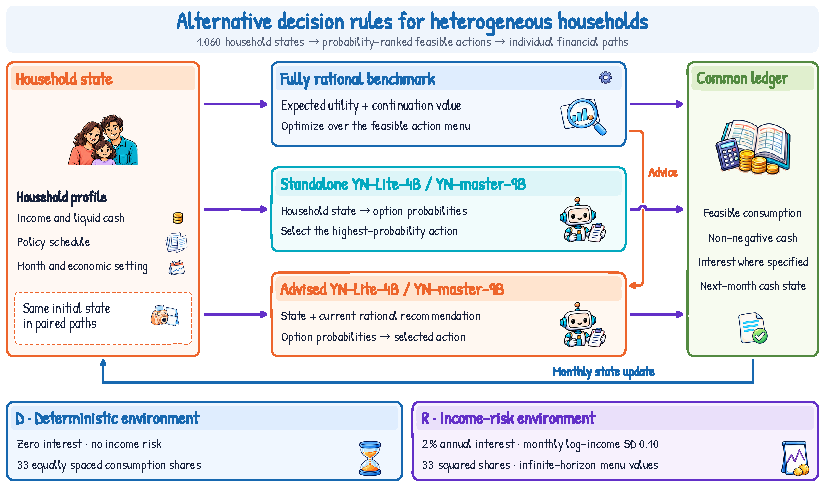
\includegraphics[width=\textwidth]{figures/household_scenario.pdf}
\caption{\textbf{Standalone and advised learned policies share a household accounting interface.} The fully rational benchmark optimizes consumption and saving. Standalone policies map household information directly to candidate probabilities; advised policies additionally receive a rational recommendation evaluated at their own current cash state. Argmax selects a feasible action and the ledger advances the household. Standalone results are available in D; rational and advised comparisons are available in both D and R, using the same households and annual evaluation target.}
\label{hh:fig:scenario}
\end{figure}

The deterministic specification, D, used zero interest, constant income and 33 equally spaced consumption shares $s_k=k/32$. The income-risk specification, R, used a 2\% annual real interest rate, uncertain future income and shares $s_k=(k/32)^2$, concentrating options at low consumption rates. Both used $k=0,\ldots,32$. Standalone models and both advised models were evaluated in D; the rational benchmark and both advised models were also evaluated in R. Each specification retains its recorded price convention: D amounts are nominal, whereas R amounts are converted from reference-year prices by dividing by 0.964311. This conversion accounts for the reported income components of 221.12 and 229.31 yuan. D and R compare complete specifications that change prices, interest, risk and the menu together.

The household experiment used the head-only 200k YN-Lite-4B variant: Qwen3.5-4B-Base remained frozen while its decision head was trained. This differs from the LoRA-plus-head 4B checkpoint selected for the benchmark in Section 4.3. YN-master-9B used the selected LoRA-adapted Qwen3.5-9B. Each interface returned probabilities over all 33 candidates; the highest-probability feasible candidate determined consumption. In advised runs, the rational recommendation was recomputed each month at the learned policy's own cash state.

\clearpage
\subsection*{7.2. Standalone policies predicted annual consumption with distinct distributional errors}

We evaluated the forecasts against observed annual consumption, using fixed household weights and 2018 nominal yuan. Annual predictions combined eight-twelfths of pre-policy annual consumption with the four simulated months. This shared prefix is an assigned pre-announcement consumption level, not an observed eight-month outcome:
\begin{equation}
 \widehat C_i=\frac{8}{12}C_i^{\mathrm{pre}}+\sum_{t=9}^{12}c_{it}^{\mathrm{policy}}.
 \label{hh:eq:annual}
\end{equation}
Income and net wealth, each divided by the square root of household size, defined separate weighted tertiles before model evaluation. For normalized weights $w_i$, group mass $W_g=\sum_{i\in g}w_i$ and observed annual consumption $C_i$, group fit was
\begin{equation}
 D=\left(\sum_{g=1}^{3}W_g\mu_g^2\right)^{1/2},\qquad
 \mu_g=\sum_{i\in g}\frac{w_i}{W_g}\left[\log(1+\widehat C_i)-\log(1+C_i)\right].
 \label{hh:eq:group}
\end{equation}
MAE and RMSE summarized household-level amount errors; income and wealth $D$ summarized the weighted root-mean-square of the group mean log errors, including overall prediction bias. Table~\ref{hh:tab:group-mae} additionally reports within-tertile MAE, averaging absolute household errors separately in each income and wealth group.

\begin{table}[H]
\centering\footnotesize
\setlength{\tabcolsep}{3.5pt}
\begin{tabularx}{\textwidth}{@{}Xrrrrr@{}}
\toprule
Decision rule & MAE & RMSE & Predicted mean & Income $D$ & Wealth $D$\\
\midrule
Rational benchmark (D) & 53,128.42 & 139,410.00 & 92,840.11 & 0.19283 & 0.07147\\
Standalone YN-Lite-4B (D) & 53,989.67 & 136,065.36 & 90,543.88 & 0.16533 & 0.08471\\
Standalone YN-master-9B (D) & 51,312.38 & 135,018.99 & 79,745.82 & 0.20688 & 0.16664\\
Advised YN-Lite-4B (D) & 54,899.68 & 135,972.02 & 92,809.03 & 0.17723 & 0.07424\\
Advised YN-master-9B (D) & 53,103.68 & 139,384.72 & 93,083.54 & 0.19104 & 0.07129\\
\midrule
Rational benchmark (R) & 54,650.51 & 140,118.28 & 98,300.12 & 0.20730 & 0.10311\\
Advised YN-Lite-4B (R) & 54,601.82 & 140,107.74 & 96,818.73 & 0.19621 & 0.08966\\
Advised YN-master-9B (R) & 54,636.46 & 140,109.03 & 98,276.71 & 0.20714 & 0.10279\\
\midrule
Continuous rational reference (D) & 52,880.93 & 138,521.14 & 91,940.42 & 0.18880 & 0.06272\\
Continuous rational reference (R) & 54,588.50 & 139,751.83 & 98,168.47 & 0.20689 & 0.10189\\
\midrule
Standalone YN-mini (D) & 72,429.94 & 173,019.10 & 116,041.44 & 0.23321 & 0.17079\\
Advised YN-mini (D) & 67,301.29 & 166,334.61 & 105,796.50 & 0.17193 & 0.11323\\
\midrule Pre-policy consumption carried forward & 52,420.72 & 138,162.11 & -- & -- & --\\
\bottomrule
\end{tabularx}
\caption{\textbf{Annual consumption forecasts for 1,060 households.} Amounts are household-weighted 2018 nominal yuan; the observed mean is 99,300.73 yuan. D denotes the deterministic specification and R the income-risk specification. Comparisons within each specification share the economic environment and menu. Continuous solutions and the 421M variants are included as references. Carry-forward predicts each household's pre-policy consumption without a simulated decision path.}
\label{hh:tab:complete}
\end{table}

Standalone YN-master-9B had the lowest annual MAE and RMSE among the evaluated systems. Against the deterministic rational benchmark, its MAE fell by 3.42\% and RMSE by 3.15\%. Relative to carrying pre-policy consumption forward, MAE was 2.11\% lower and RMSE 2.27\% lower. Its predicted population mean was 79,746 yuan, compared with an observed 99,301 yuan, and its income- and wealth-group distances exceeded the benchmark's. The mean signed error was negative in all six tertiles. Its MAE advantage was concentrated in the highest income group (83,282 versus 90,874 yuan), while the low- and middle-income group errors were higher (Table~\ref{hh:tab:group-mae}). Lower individual amount error therefore coexisted with a systematic downward bias.

Standalone YN-Lite-4B had lower mean log prediction bias across income tertiles. Its income-group distance was 14.26\% lower than the deterministic rational benchmark's and its RMSE was 2.40\% lower, whereas MAE was 1.62\% higher and wealth-group distance was 18.52\% higher. Figure~\ref{hh:fig:results} shows these differences in individual and group prediction errors.



Advice moved the 9B forecast toward the rational benchmark. Under D, its predicted mean rose from 79,746 to 93,084 yuan and wealth $D$ fell from 0.16664 to 0.07129, while MAE rose to 53,103.68 yuan. Under R, advised YN-master-9B closely tracked the benchmark. Advised YN-Lite-4B reduced income and wealth $D$ by 5.35\% and 13.04\% relative to the R benchmark, with an MAE reduction of 0.089\%.

\clearpage
\begin{figure}[H]
\centering
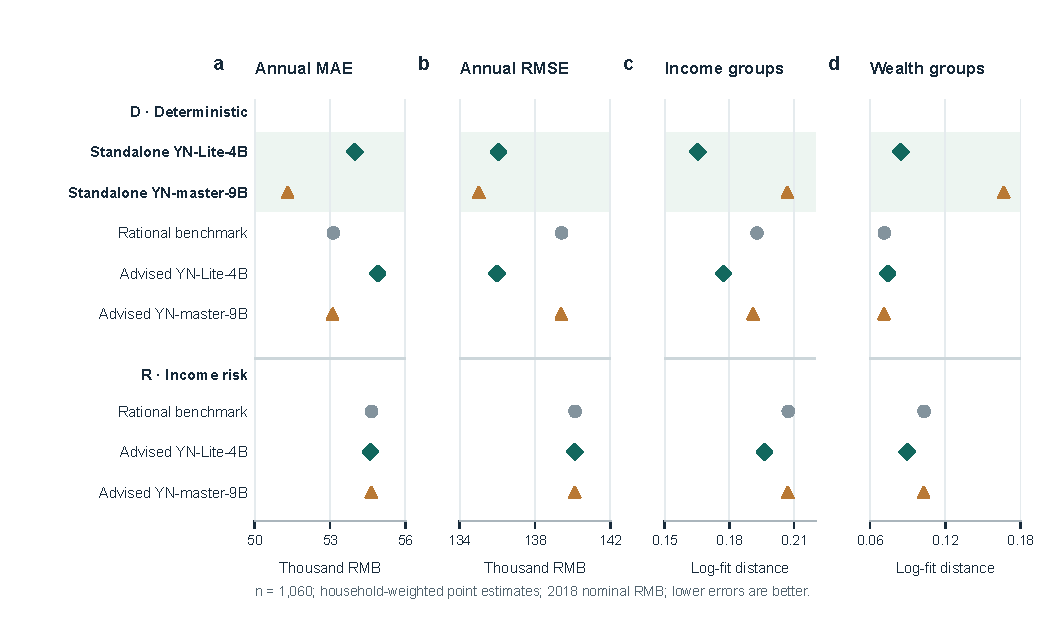
\includegraphics[width=\textwidth]{figures/household_main_results.pdf}
\caption{\textbf{Standalone policies and rational advice produce different prediction profiles.} Annual MAE, RMSE and income- and wealth-group log-fit distances for the eight principal systems. The two specifications are separated: D uses deterministic income and an equally spaced menu; R includes income risk and a squared-share menu. All forecasts use the same households, weights, price units and observed annual target. Lower values indicate closer fit.}
\label{hh:fig:results}
\end{figure}
\subsection*{7.3. Household-specific optimization provides a common rational baseline}

Following Kaplan et al.'s consumption--saving household approach~\cite{ref32}, the R benchmark used CRRA utility $u(c)=c^{1-\gamma}/(1-\gamma)$, $\gamma=2$, monthly discounting $\beta_m=0.96^{1/12}$ and return $R_m=1.02^{1/12}$. Future income multipliers were independent mean-one lognormal draws with log standard deviation $0.10$; recorded paths realized their conditional mean. For resources $m$, regular income $\bar y_i$ and policy component $g_{i,t+1}$, the rational policy solved
\begin{equation}
 V_{it}(m)=\max_{s\in\mathcal S}\left\{u(sm)+\beta_m\mathbb{E}\left[V_{i,t+1}\!\left(R_m(1-s)m+\bar y_i\varepsilon_{t+1}+g_{i,t+1}\right)\right]\right\}.
 \label{hh:eq:bellman}
\end{equation}
The solver optimized all 33 shares on a 4,096-point resource grid with seven income-risk quadrature nodes and infinite-horizon same-menu continuation. A continuous endogenous-grid solution~\cite{ref43} supplied the numerical reference. The D benchmark selected $\beta_m$ over $[0.8,0.999999]$ by minimizing the household-weighted mean squared error in pre-policy monthly $\log(1+c)$; the solution reached the upper boundary. This calibration used only pre-policy consumption. D used exact continuous continuation after four menu periods.

Income and wealth groups defined evaluation strata; optimization used each household's income, cash and policy component with common preferences. R parameters were fixed before outcome scoring. Within each specification, the rational economic agent and learned policies faced the same menu, income schedule, cash constraint and accounting equations.

\subsection*{7.4. Future-information tests reveal when model decisions change}

The primary annual forecasts used anonymous policy inputs without later outcome notes. We tested sensitivity to added information in two separate designs. A fixed 64-household panel held September states and menus constant while adding a historical policy label, two later consumption--exposure regression slopes from the full 1,060-household sample, or the same slopes with reversed signs (Figure~\ref{hh:fig:information}). It covered standalone/advised consumption choices and direct annual-consumption and December-cash questions. The 120 policy-only inputs omitted household profiles and varied an anonymous description, a historical year, a future-year relabeling, and synthetic positive or negative retrospective claims. Each model answered three question types under five information conditions, two equivalent wordings and two option orders.

\clearpage
\begin{figure}[H]
\centering
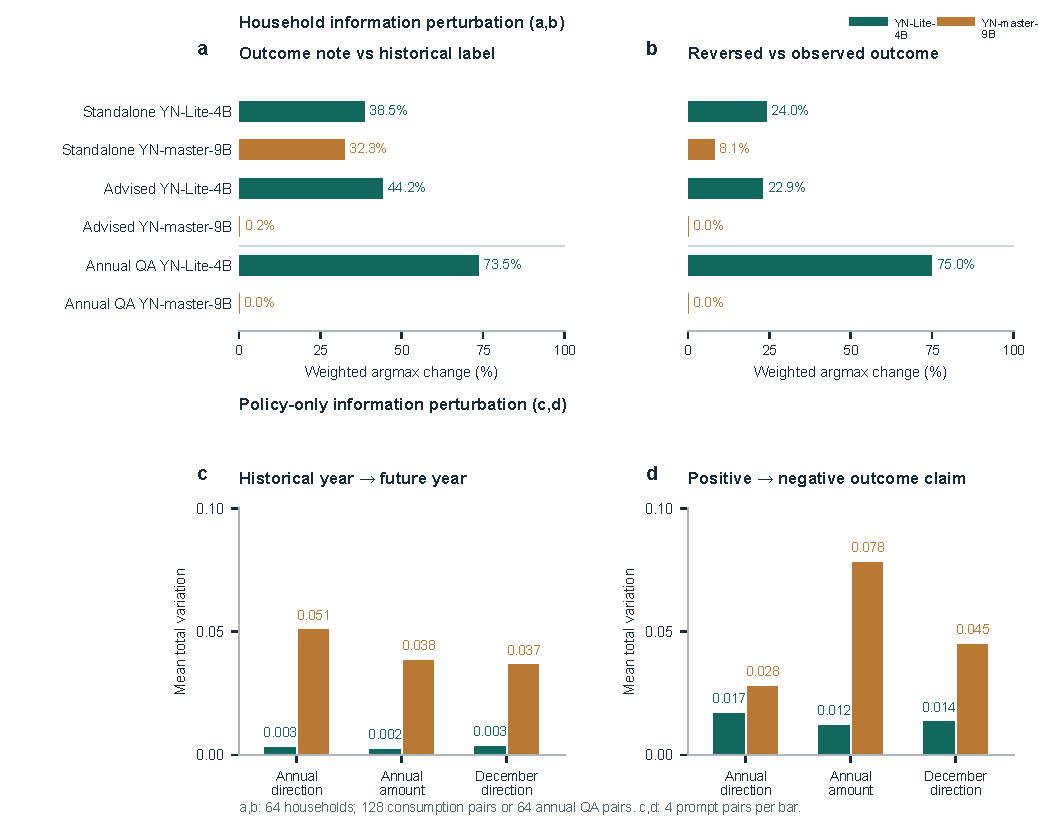
\includegraphics[width=\textwidth]{figures/household_information.pdf}
\caption{\textbf{Decision sensitivity depends on both the model and the information task.} \textbf{a,b,} The outcome note supplied two adjusted weighted-regression slopes linking the observed pre-policy-to-outcome-year change in real $\log(1+C)$ to predicted fourth-quarter tax-income gains in the full 1,060-household sample: $-0.05375229$ for high-liquidity households and $-0.05404250$ for low-liquidity households, per 1,000 yuan of exposure. These are descriptive associations conditional on household covariates. Panel a adds this note to the historical-label input; panel b reverses both signs. Consumption comparisons contain 128 pairs (64 households in two income paths); direct annual-direction questions contain 64. Rates use household weights. \textbf{c,d,} Policy-only tests compare historical and future year labels, and positive and negative synthetic retrospective claims. Total variation is $\tfrac12\sum_k|p_k-q_k|$; each cell averages four wording/order pairs.}
\label{hh:fig:information}
\end{figure}

Observed later statistics altered standalone consumption choices in 57 of 128 comparisons for YN-Lite-4B and 38 of 128 for YN-master-9B. With rational advice, the corresponding counts were 45 and 1. Reversing the statistics changed 32 standalone 4B choices and 7 standalone 9B choices. Direct annual-direction questions were especially responsive for 4B: the observed note changed 48 of 64 answers, and reversing it changed 50. The 9B annual-direction argmax remained unchanged in both comparisons, although its mean weighted probability shifts were 0.04624 and 0.05035 in total variation.



In policy-only questions, YN-Lite-4B selected ``cannot determine'' in all 60 inputs. YN-master-9B selected an increase in all 40 direction questions; for annual magnitude, it selected ``cannot determine'' in 19 of 20 cases and a change within $\pm0.1\%$ once. Relabeling the policy year from 2018 to 2031 left the selected choices unchanged in all 12 paired tests per model, while moving the 9B annual-direction distribution by mean TV 0.05075 and the December-direction distribution by 0.03659. Reversing the synthetic retrospective claim changed its annual-magnitude distribution by 0.07819 and flipped one of four choices. Equivalent wording and reversed option order each changed one of 30 paired 9B choices and no 4B choices. These interventions measure decision sensitivity to supplied dates and outcome claims; they do not measure what the training corpus contains.

\clearpage
\subsection*{7.5. Interpretation: An alternative policy module with distinct consumption--cash behavior}

These results support learned decision rules as another route to large heterogeneous-agent simulation. A shared trained policy maps household profiles and budgets to feasible actions, while the simulator updates financial states. The contrast between 9B's lower individual error and 4B's smaller income-tertile mean log errors makes both levels of evaluation relevant as the simulated population becomes more heterogeneous.

The standalone 9B underprediction arises from lower selected consumption and greater cash retention. At identical September states, it chose a lower consumption share than the deterministic rational benchmark for 65.8\% of household weight; mean selected shares were 25.8\% and 38.4\%. Its four-month consumption totaled 30,141 yuan versus 43,235 yuan, leaving 13,094 yuan more in December cash. Added to the common 49,605-yuan eight-month prefix, this produced the 79,746-yuan annual forecast, 19.7\% below the observed mean. Rational advice raised four-month consumption to 43,478 yuan and narrowed the annual gap.

Paired policy increments compare two independently simulated September--December paths for each household and decision rule. Both start from the same initial state: the baseline retains the original tax schedule, while the policy path includes the tax-cut income component announced in September and paid from October. Each path updates consumption and cash monthly. We subtract baseline from policy within each household, then average these paired differences with household weights.

In R, the income component provided 229.31 yuan over October--December. Advised YN-Lite-4B allocated 19.23 yuan to additional consumption and 210.42 yuan to closing cash, retaining about 92\% of the component. Advised YN-master-9B increased consumption by 271.30 yuan and reduced cash by 42.22 yuan, close to the rational benchmark's allocation (Figure~\ref{hh:fig:allocation}). In D, standalone YN-Lite-4B increased consumption by 502.78 yuan, whereas standalone YN-master-9B reduced it by 904.38 yuan and accumulated 1,125.51 yuan in cash. Thus the 9B policy's favorable annual prediction score accompanied a negative simulated consumption response to the income component.

\begin{figure}[H]
\centering
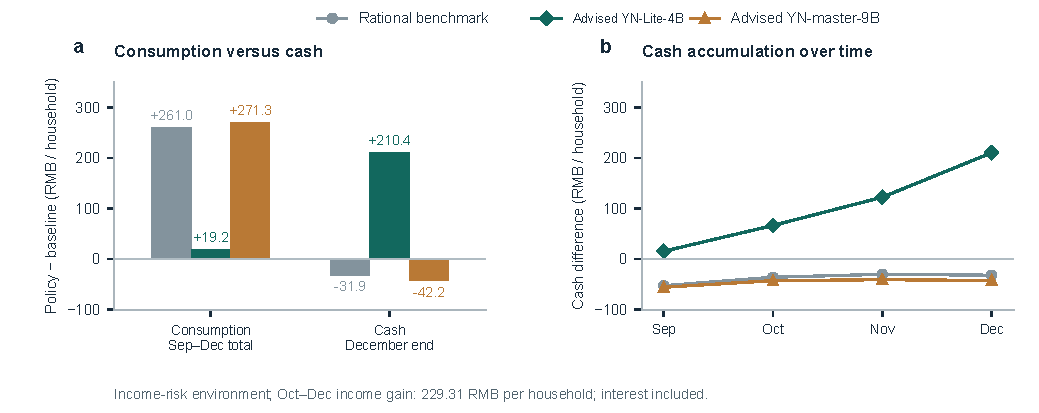
\includegraphics[width=\textwidth]{figures/household_policy_allocation.pdf}
\caption{\textbf{Conditional income gains are allocated differently between consumption and cash.} The income-risk specification compares the fully rational benchmark with advised 4B and 9B. All changes are policy minus baseline: consumption is summed over September--December, whereas cash is the December-end stock. The right panel tracks month-end cash differences. Amounts are household-weighted 2018 nominal yuan. Table~\ref{hh:tab:channels} gives all decision rules.}
\label{hh:fig:allocation}
\end{figure}

The common budget connects these responses through
\begin{equation}
 \Delta C_{9:12}+\Delta a_{13}=\sum_{t=9}^{12}\Delta g_t+\Delta I_{9:12}.
 \label{hh:eq:budget}
\end{equation}
The component totals were 221.12 yuan in D and 229.31 yuan in R in common price units.



\clearpage
\subsection*{7.6. Complete group, information and consumption--cash results}
\begingroup
\setlength{\intextsep}{5pt}
\captionsetup{font=footnotesize,skip=3pt}
\begin{table}[H]
\centering\footnotesize
\setlength{\tabcolsep}{3pt}
\begin{tabularx}{\textwidth}{@{}Xrrrrrr@{}}
\toprule
 & \multicolumn{3}{c}{Income tertile} & \multicolumn{3}{c}{Wealth tertile}\\
\cmidrule(lr){2-4}\cmidrule(l){5-7}
Decision rule & Low & Middle & High & Low & Middle & High\\
\midrule
Rational benchmark (D) & 28,023 & 40,908 & 90,874 & 34,949 & 60,060 & 64,540\\
Standalone YN-Lite-4B (D) & 29,435 & 45,778 & 87,109 & 35,864 & 62,477 & 63,795\\
Standalone YN-master-9B (D) & 29,564 & 41,443 & 83,282 & 34,856 & 59,530 & 59,704\\
Advised YN-Lite-4B (D) & 30,348 & 44,303 & 90,438 & 37,097 & 65,836 & 61,933\\
Advised YN-master-9B (D) & 27,807 & 41,050 & 90,873 & 34,765 & 60,093 & 64,619\\
\midrule
Rational benchmark (R) & 27,192 & 41,772 & 95,438 & 35,625 & 60,765 & 67,731\\
Advised YN-Lite-4B (R) & 27,377 & 41,993 & 94,880 & 35,701 & 60,677 & 67,595\\
Advised YN-master-9B (R) & 27,189 & 41,779 & 95,392 & 35,619 & 60,770 & 67,690\\
\midrule
Continuous rational reference (D) & 28,029 & 41,297 & 89,724 & 34,882 & 60,060 & 63,864\\
Continuous rational reference (R) & 27,315 & 41,795 & 95,103 & 35,639 & 60,722 & 67,573\\
\midrule
Standalone YN-mini (D) & 32,668 & 56,906 & 128,321 & 38,960 & 67,461 & 111,137\\
Advised YN-mini (D) & 30,327 & 51,342 & 120,821 & 36,892 & 64,061 & 101,197\\
\midrule
Pre-policy consumption carried forward & 31,040 & 43,808 & 82,744 & 35,499 & 61,191 & 60,728\\
\bottomrule
\end{tabularx}
\caption{\textbf{Annual MAE within income and wealth tertiles.} Household-weighted 2018 nominal yuan, rounded to the nearest yuan. Each cell is $\mathrm{MAE}_g=\sum_{i\in g}(w_i/W_g)|\widehat C_i-C_i|$. Income groups contain 337/338/385 households; wealth groups contain 351/308/401. Group weights reconstruct each rule's overall MAE.}
\label{hh:tab:group-mae}
\end{table}

\begin{table}[H]
\centering\footnotesize
\begin{tabularx}{\textwidth}{@{}lXrrr@{}}
\toprule
Model & Fixed-household task & Historical label & Outcome note & Reversed note\\
\midrule
4B & Standalone consumption & 42/128 & 57/128 & 32/128\\
4B & Advised consumption & 36/128 & 45/128 & 30/128\\
4B & Annual consumption direction & 14/64 & 48/64 & 50/64\\
4B & December cash direction & 21/64 & 20/64 & 37/64\\
\midrule
9B & Standalone consumption & 16/128 & 38/128 & 7/128\\
9B & Advised consumption & 1/128 & 1/128 & 0/128\\
9B & Annual consumption direction & 0/64 & 0/64 & 0/64\\
9B & December cash direction & 17/64 & 7/64 & 1/64\\
\midrule
421M & Standalone consumption & 20/128 & 8/128 & 4/128\\
421M & Advised consumption & 13/128 & 11/128 & 0/128\\
421M & Annual consumption direction & 0/64 & 0/64 & 0/64\\
421M & December cash direction & 0/64 & 0/64 & 0/64\\
\bottomrule
\end{tabularx}
\caption{\textbf{Changed choices in the fixed-household information test.} Entries are unweighted flips/pairs. Historical label is compared with the anonymous input; observed outcome information is compared with the historical label; the reversed note is compared with the observed note. Consumption tasks include both paths at the same initial household state. The 421M reference used the same 64-household design.}
\label{hh:tab:information}
\end{table}
\begin{table}[H]
\centering\footnotesize
\begin{tabularx}{\textwidth}{@{}Xrrr@{}}
\toprule
Decision rule & $\Delta C_{9:12}$ & $\Delta a_{13}$ & $\Delta I_{9:12}$\\
\midrule
Rational benchmark (D) & +249.58 & -28.46 & +0.00\\
Standalone YN-Lite-4B (D) & +502.78 & -281.66 & +0.00\\
Standalone YN-master-9B (D) & -904.38 & +1,125.51 & +0.00\\
Advised YN-Lite-4B (D) & -645.67 & +866.79 & +0.00\\
Advised YN-master-9B (D) & +193.22 & +27.90 & +0.00\\
\midrule
Rational benchmark (R) & +260.97 & -31.86 & -0.20\\
Advised YN-Lite-4B (R) & +19.23 & +210.42 & +0.34\\
Advised YN-master-9B (R) & +271.30 & -42.22 & -0.23\\
\midrule
Continuous rational reference (D) & +292.58 & -71.46 & +0.00\\
Continuous rational reference (R) & +308.42 & -79.50 & -0.38\\
\midrule
Standalone YN-mini (D) & -2,006.08 & +2,227.20 & +0.00\\
Advised YN-mini (D) & -8,962.40 & +9,183.53 & +0.00\\
\bottomrule
\end{tabularx}
\caption{\textbf{Paired consumption and cash changes.} Policy minus baseline, in household-weighted 2018 nominal yuan. Cash is the December-end stock; consumption and interest are four-month totals. D and R retain their original economic specifications and component paths.}
\label{hh:tab:channels}
\end{table}
\endgroup
